\documentclass{article}
\usepackage[utf8]{inputenc}
\usepackage[T1]{fontenc}
\usepackage{graphicx}
\usepackage{hyperref}
\usepackage{geometry}
\geometry{margin=1in}

\title{COMITA}
\date{Encyclopaedia Britannica (1771)}

\begin{document}
\maketitle

\section*{Historical source}
\textbf{Entry ID:} \texttt{entry-comita-1102} \\
\textbf{Volume ID:} 193109114 \\
\textbf{Character Count:} 4530

\subsection*{Extracted Text}
COMITA, in Roman University, general assemblies of the people, covered by a registered for the purpose of putting any subjects to their vote.

The proper combina were of three sons \_and certain, contra\_- rivals, and tribute, with reference to the three grand divisions of the city and people in \_nurcarta\_, centuries, and critics far y cowmila celebrity men meant all the coming general, the term colonism (from editor, i.e., courtesy), being their common epithet, though it was at last restricted to assemblies for the creation of priests, and the regulation of lat wills and tenaments, to which the people acted as witnesses merely.

The comitia curvida owed its origin to the division which Romulus made of the people into thirty curtu, ten being consumed in every tribe. The curtu answered the next te- aspects to the problem is our cities, being not only separated by proper bounds and limits, but distinguished too by the different places set apart in each for the celebration of religious service, which was performed by particular priest called \_extremely,\_ one to every citizen.

Before the institution of the comitia contents, all the great concerts of the state were transacted in the assembly of the curtu; as the election of kings and other chief officers, the major and beginning of lives, and the judging of qui- ultricutes. After the repetition of the Bishop, when the commons had obtained the privilege of bring tribune and thus, they were the ones now elected at these assemblages, but that ceremony being at length transferred to the comitia tribus, the curtu were never converted to give their votes, reception venue, and making some particular law, relating to an adaptation, walls, and treatments, or the creation of officers for an exposition, for elective, some of the priets, as the famines, and the new maratons, who were four-selves chosen by every particular curtu. The power of calling these was clearly believed at that only to the knayy, but to the establishment of the democracy, this privilege was allowed to most of the magistrates, and sometimes to the positionities.

The parents who had all liberty of voting over such Romans citizens and belonged to the curtu, or actually lived in the city, and confirmed to the customs and their of their proper cursu and all were excluded who dwell without the bounds of the city, or retained the ceremonies of their own country even, although they had been consumed with the \_ja créaviside\_ (See Grimes). The place where the cursus met was the conditions a pard of the forum. No fixed time was appointed for holding pay of the comitia, but they were conversed as business required.

The people being met together, and murted by the request of good news from the magnent, which may necessary in all the assemblies, the cognitive business to be proposed to them was publicly read. After this, if none of the misti- trates requested, upon the order of him who presided in the comitia, the people divided into their proper cursu, and can be pulled off the matters and then the curtu being called out, as it happened by lot, gave their votes man by man, in ancient times were now, and afterwards by tables; the most votes in every curts going for the voice of the whole curtu, and the most curlar for the general consent of the people.

In the time of Clover, the comitia curtains were a much out of isolation that they were formed only only thirty literary representing the thirty curtu; instance, in his second ex-tion region Rulls, the calls them commitate indefinite.

The comitia center was inserted by Servita Tul-lia, who had obliged every one to give a time account of that he has saved, and divided the people, according to the returns, that six rows or cases, which is subdivided into a hundred and minety-three centuries. The first class, containing the copies and indeed citizens, consisted of ninety-seven centuries, the third of twenty-the fourth of twenty-two, the fifth thirty; did the study, composed of the persort, and only one century, but this thought it had the same name with the rest, yet was seldom regarded, and scarcely allowed any power in public matter. Hence it is common with the Roman authors, when they speak of the classes to action no means than the skills to being used their notice. She has classanted orders and divided into two parts or entries, the protectorii and the capite coast. The former, as their name implies, were designed purely to stock the republic with men, since they could supply it with so little money i



\section*{Source record}
\begin{itemize}
\item \textbf{Dataset:} \texttt{NationalLibraryOfScotland/encyclopaedia\_britannica\_illustrated}
\item \textbf{Dataset Revision:} \texttt{309f765b1ecc83e0a7f7762e44b4a927a7555443}
\item \textbf{Page ID:} \texttt{britannica:309f765b1ecc83e0a7f7762e44b4a927a7555443:train:1102} \\
  \textbf{Filename:} \texttt{page-1102-918dd1676cc2.jpg} \\
  \textbf{Row Index:} 1102 \\
  \textbf{SHA256:} \texttt{918dd1676cc2e629...}
\end{itemize}

\begin{figure}[h]
\centering
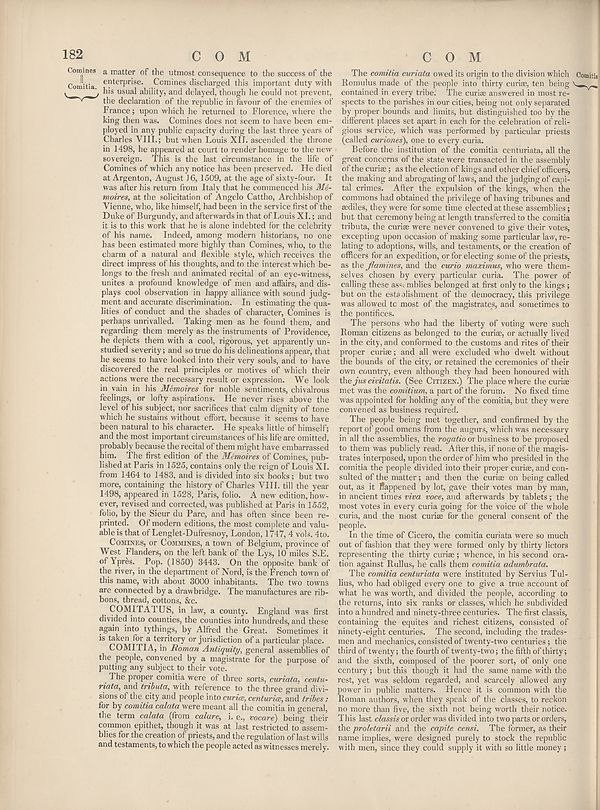
\includegraphics[width=0.85\textwidth]{../scans/page-1102-918dd1676cc2.jpg}
\caption*{Source scan: \texttt{page-1102-918dd1676cc2.jpg}}
\end{figure}

\end{document}
